%%%%%%%%%%%%%%%%%%%%%%%%%%%%%%%%%%%%%%%%%%%%%%%%%%%%%%%%%%%%%%%%%%%%%%%%%%%%%%%%
% SD Lab -- Topic
% Giovanni Ciatto
% Alma Mater Studiorum - Università di Bologna
% mailto:giovanni.ciatto@unibo.it
% mailto:matteo.magnini@unibo.it
%%%%%%%%%%%%%%%%%%%%%%%%%%%%%%%%%%%%%%%%%%%%%%%%%%%%%%%%%%%%%%%%%%%%%%%%%%%%%%%%
%\documentclass[handout]{beamer}\mode<handout>{\usetheme{default}}
%
\documentclass[presentation]{beamer}\mode<presentation>{\usetheme{AMSBolognaFC}}
%\documentclass[handout]{beamer}\mode<handout>{\usetheme{AMSBolognaFC}}
%%%%%%%%%%%%%%%%%%%%%%%%%%%%%%%%%%%%%%%%%%%%%%%%%%%%%%%%%%%%%%%%%%%%%%%%%%%%%%%%
\usepackage{sd-lab-common}
\usepackage{sd-lab-consensus}
%%%%%%%%%%%%%%%%%%%%%%%%%%%%%%%%%%%%%%%%%%%%%%%%%%%%%%%%%%%%%%%%%%%%%%%%%%%%%%%%
\title[\currentLab{7} -- Consensus]{
	Consensus
}
%
\subtitle{\courseName{} (\courseAcronym) / Module \moduleN{}}
%
\author[\sspeaker{\mmShort} \& \gcShort]{
	\speaker{\mmFull} \and \gcFull
	\\ 
	\mmEmail \and \gcEmail
}
%
\institute[\disiShort, \uniboShort]{\disi{} (\disiShort)\\\unibo}
%
\date[A.Y. \academicYear{}]{Academic Year \academicYear{}}
%
%%%%%%%%%%%%%%%%%%%%%%%%%%%%%%%%%%%%%%%%%%%%%%%%%%%%%%%%%%%%%%%%%%%%%%%%%%%%%%%%
\begin{document}
%%%%%%%%%%%%%%%%%%%%%%%%%%%%%%%%%%%%%%%%%%%%%%%%%%%%%%%%%%%%%%%%%%%%%%%%%%%%%%%%

%/////////
\frame{\titlepage}
%/////////

%%===============================================================================
\section*{Outline}
%%===============================================================================
%
%%/////////
\frame[c]{\tableofcontents[hideallsubsections]}
%%/////////

%===============================================================================
\section{Goals and theory recall}
%===============================================================================

\begin{frame}{Lecture Goals}
	\begin{itemize}
		\item Be familiar with consensus and know at least one ``simple'' consensus algorithm (raft);
        %
        \item Usage of the \emph{etcd} technology: etcd servers for a replicated key-value store based on raft;
        %
        \item Usage of the \emph{jetcd} technology: a java etcd client library.
	\end{itemize}
\end{frame}

\begin{frame}[allowframebreaks]{Theory}
    \begin{block}{Not a good start}
    	\begin{itemize}
            \item CAP theorem, what do we choose?;
            %
    		\item ``Impossibility of distributed consensus with one faulty process'' also known as the FLP theorem \ccite{FLP}, how do we make it possible?\\
            $\rightarrow$ asynchronous deterministic protocols are impossible;
            %
            \item check slides C2 -- The Problem of Consensus in Distributed Systems if you don't remember.
    	\end{itemize}
    \end{block}

    \framebreak

    \begin{block}{Time}
    	\begin{itemize}
    		\item (Full) synchrony $\rightarrow$ each message between correct nodes is delivered within a time interval $\Delta$;
            %
            \item Eventual synchrony $\rightarrow$ the system becomes (full) synchronous after one unknown point in time (Global Stabilisation Time);
            %
            \item Partial synchrony $\rightarrow$ the system is synchronous but $\Delta$ is unknown;
            %
            \item Weak synchrony $\rightarrow$ $\Delta$ can increase over time $t$ (at most polynomially);
            %
            \item Asynchrony $\rightarrow$ no time assumption on message delivery, i.e. eventually a message will be delivered.
    	\end{itemize}
    \end{block}

    \framebreak

    \begin{block}{Faults}
        In the real world things are far from ideals.
        %
        There could be faults of any sort for any reason.
        %
        When designing a consensus algorithm one should consider:
        %
        \begin{itemize}
            \item \alert{Crash} fault tolerant $\rightarrow$ a node stop working or its messages are not delivered;
            %
            \item \alert{Byzantine} fault tolerant (BFT)~\ccite{byzantine1982} $\rightarrow$ a node start behaving unpredictably (it can also be malicious).
            %
            Theoretical limit of tolerance is $N \ge 3F + 1$.
        \end{itemize}
    \end{block}

    \framebreak

    \begin{block}{Famous consensus algorithms}
        \begin{itemize}
            \item Paxos \ccite{paxos} $\rightarrow$ synchronous, crash fault tolerant, difficult to understand;
            %
            \item Raft \ccite{raft} $\rightarrow$ synchronous, crash fault tolerant, easy to understand;
            %
            \item SINTRA \ccite{sintra} $\rightarrow$ asynchronous, byzantine fault tolerant, bits/transaction increase $O(N^2)$;
            %
            \item HBBFT \ccite{hbbft} $\rightarrow$  asynchronous, byzantine fault tolerant, bits/transaction increase $O(N)$.
        \end{itemize}
    \end{block}
\end{frame}

%===============================================================================
\section{Raft consensus algorithm}
%===============================================================================

\begin{frame}{Properties}
    \begin{itemize}
        \item Easy to understand $\rightarrow$ authors have deliberately chosen to prioritise understandability (Occam's razor);
        %
        \item Safety or correctness $\rightarrow$ if any server has applied a particular log entry to its state machine, then no other server may apply a different command for the same log index;
        %
        \item Asymmetric or leader-base $\rightarrow$ strong leader, log entries only flow from the leader to the other serves;
        %
        \item Crash fault tolerance $\rightarrow$ $N \ge 2F + 1$ therefore $F \le \frac{N - 1}{2}$;
        %
        \item Membership changes $\rightarrow$ the system can continue to operate during changing in the set of servers.
    \end{itemize}
\end{frame}

\begin{frame}[allowframebreaks]{Model}
    
    \begin{block}{In a nutshell}
        First of all, \emph{raft} servers start electing one leader.
        %
        The leader accepts client's requests and replicates them to the other servers.
        %
        If the leader crashes, a new election starts and eventually a new leader is elected.
    \end{block}
    
    \framebreak
    
    There are three possible states for a node:
    \begin{itemize}
        \item \alert{Leader}  $\rightarrow$ handles all client requests;
        %
        \item \alert{Follower} $\rightarrow$ responds to requests from leader and candidates;
        %
        \item \alert{Candidate} $\rightarrow$ tries to be elected in the leader election phase.
    \end{itemize}

    \centering
    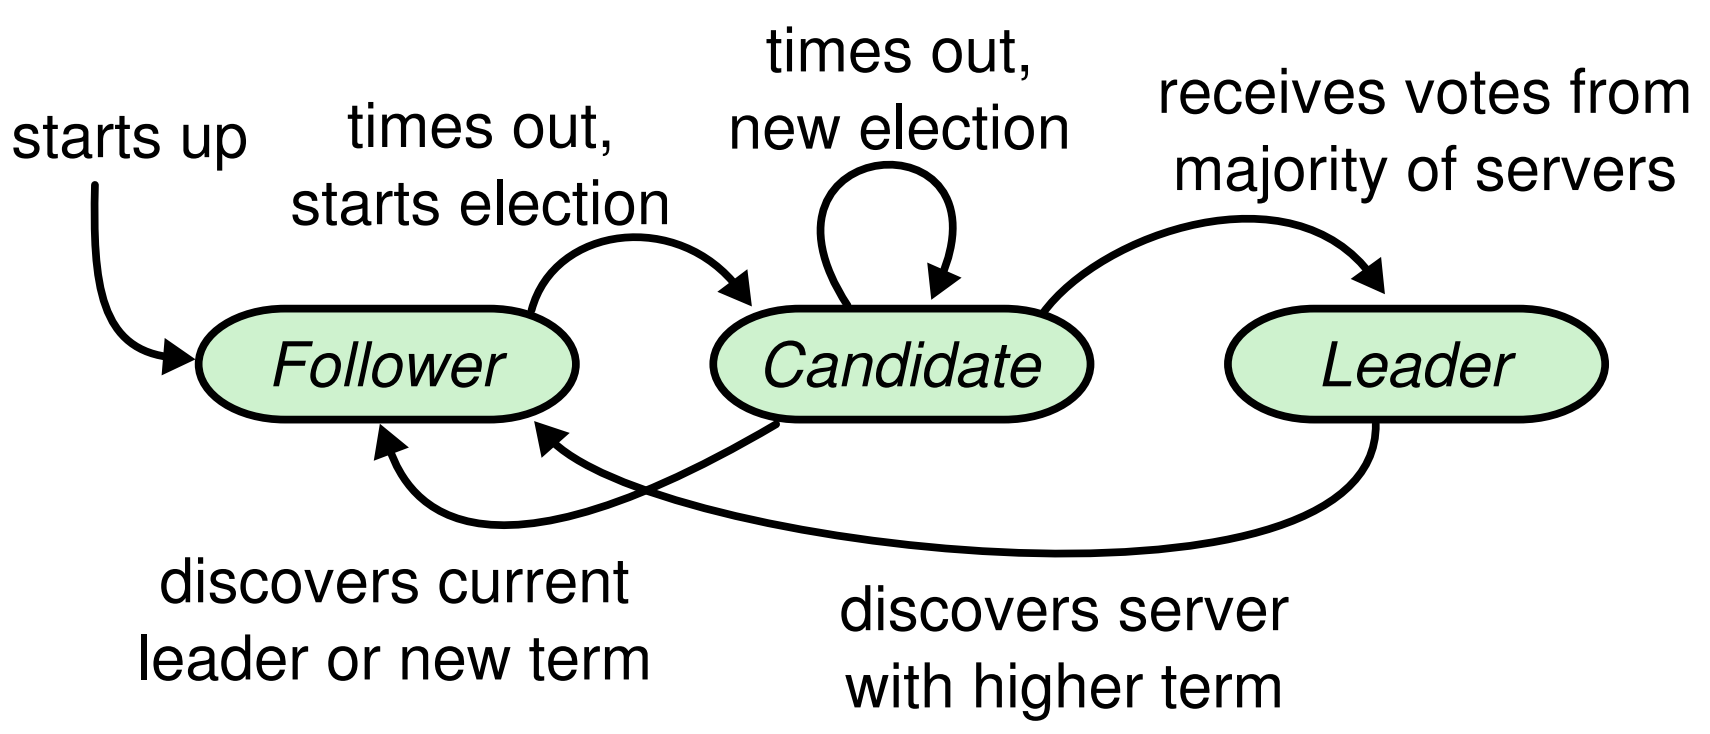
\includegraphics[width=0.8\textwidth]{figures/node-state-diagram.png}
    
    \framebreak
    
     \begin{block}{Time}
        Time is divided into \alert{\emph{terms}} of arbitrary length.
        %
        \emph{Terms} are numbered with consecutive integers.
        %
        Each \emph{term} begins with an election.
        %
        If a candidate wins it is the leader for the rest of the \emph{term}.
        %
        If the election results in a split vote the \emph{term} finishes and a new \emph{term} will begin.
    \end{block}

    \centering
    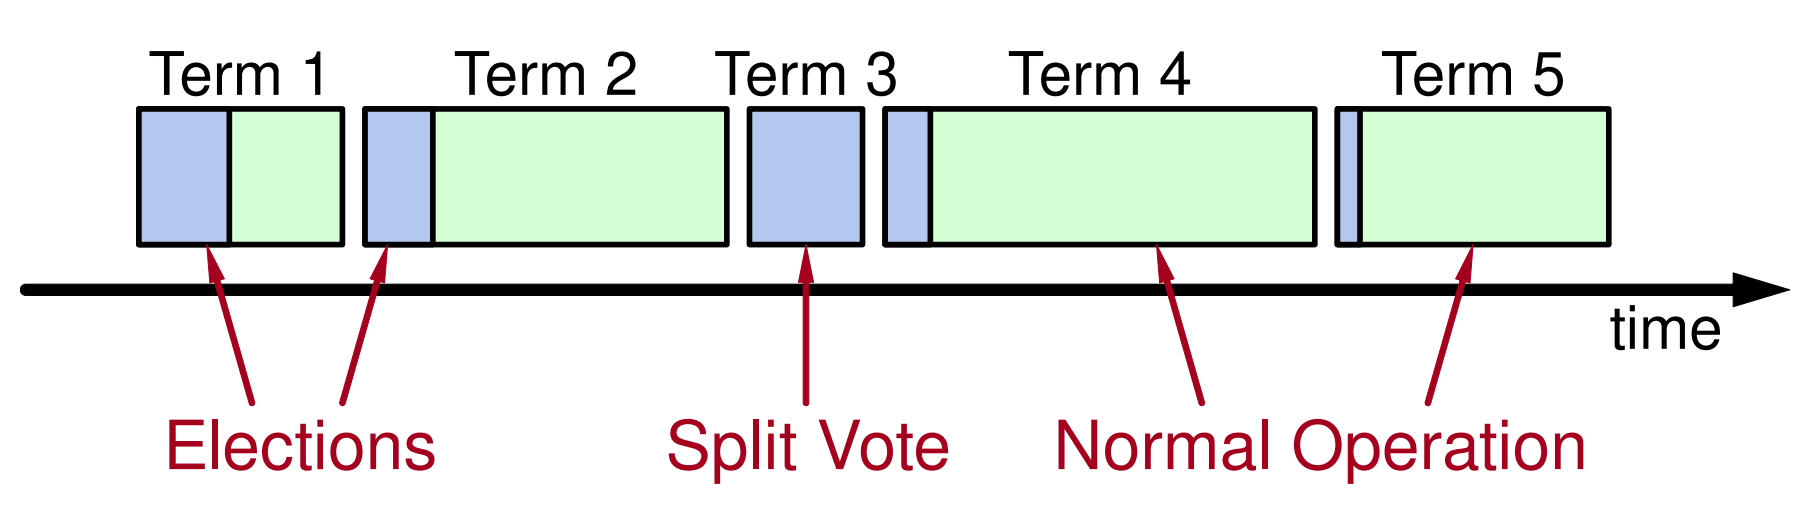
\includegraphics[width=0.8\textwidth]{figures/time.png}
    
    \framebreak
    
    \begin{block}{Leader election}
        Heartbeats are used to trigger leader election.
        %
        When a server starts it begins as \emph{follower}.
        %
        A server remains \emph{follower} as long as it receives a valid heartbeat from a \emph{leader} or \emph{candidate}.
        %
        If a \emph{follower} receives no communication over a period of time, then it assumes there is no available leader and begins an election.
        %
        A \emph{candidate} stays in this state until:
        \begin{itemize}
            \item it wins the election ($\rightarrow$ \emph{leader});
            %
            \item another server wins the election ($\rightarrow$ \emph{follower});
            %
            \item a period of time goes with no winner ($\rightarrow$ new \emph{term});.
        \end{itemize}   
 \end{block}
    
    \framebreak
    
    \begin{block}{Log replication}
        When receiving a command the \emph{leader} appends it to its log as a new entry.
        %
        Then it send the entry to the other servers for replication.
        %
        When the entry has been safely replicated, the \emph{leader} applies the entry to its state machine and returns the result of that execution to the client.
        %
        If \emph{followers} crash or run slowly, or if network packets are lost, the \emph{leader} retries.
    \end{block}

    \framebreak

    \centering
    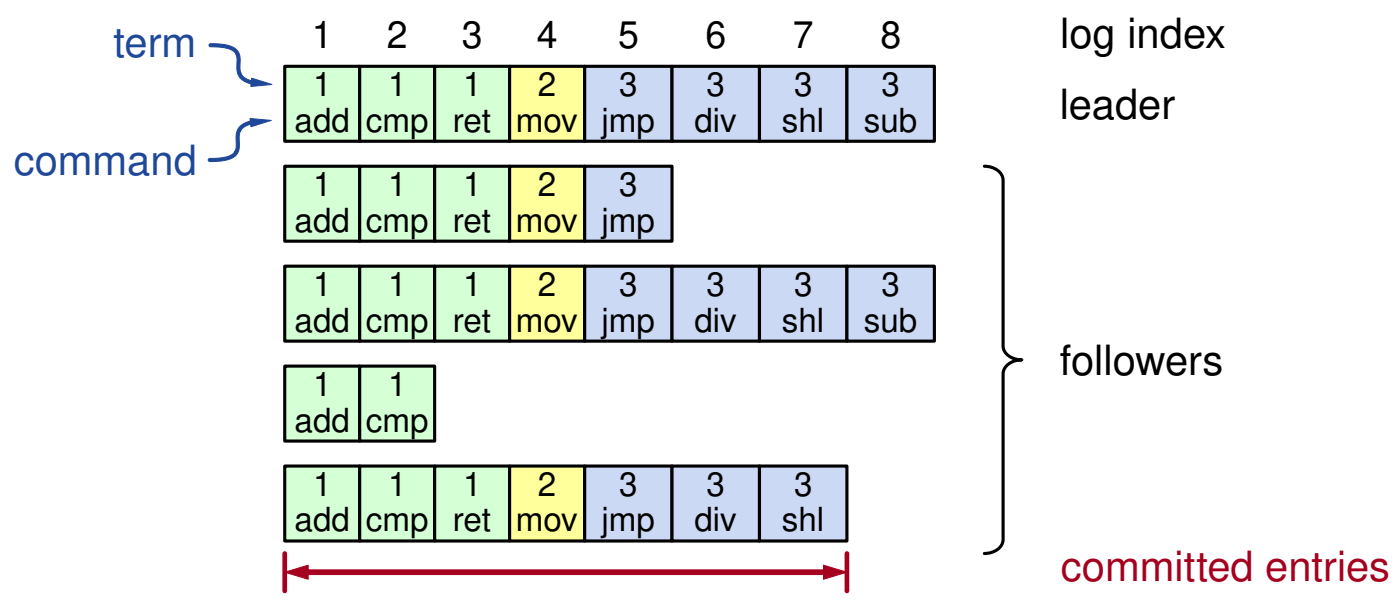
\includegraphics[width=0.8\textwidth]{figures/log.png}
    %
    \\\vspace{2em}
    Very nice web app to check your understanding: \alert{\href{https://raft.github.io/}{raft.github.io}}

\end{frame}

%===============================================================================
\section{etcd technology}
%===============================================================================

\begin{frame}[allowframebreaks]{etcd}
	\begin{block}{What is etcd?}
		``etcd is a strongly consistent, \alert{distributed key-value store} that provides a reliable way to store data that needs to be accessed by a distributed system or cluster of machines.
        %
        It gracefully handles leader elections during network partitions and can tolerate machine failure, even in the leader node.''
        %
        \begin{flushright}
            (\href{https://etcd.io/}{etcd.io})
        \end{flushright}
	\end{block}
	%
    
    \centering
    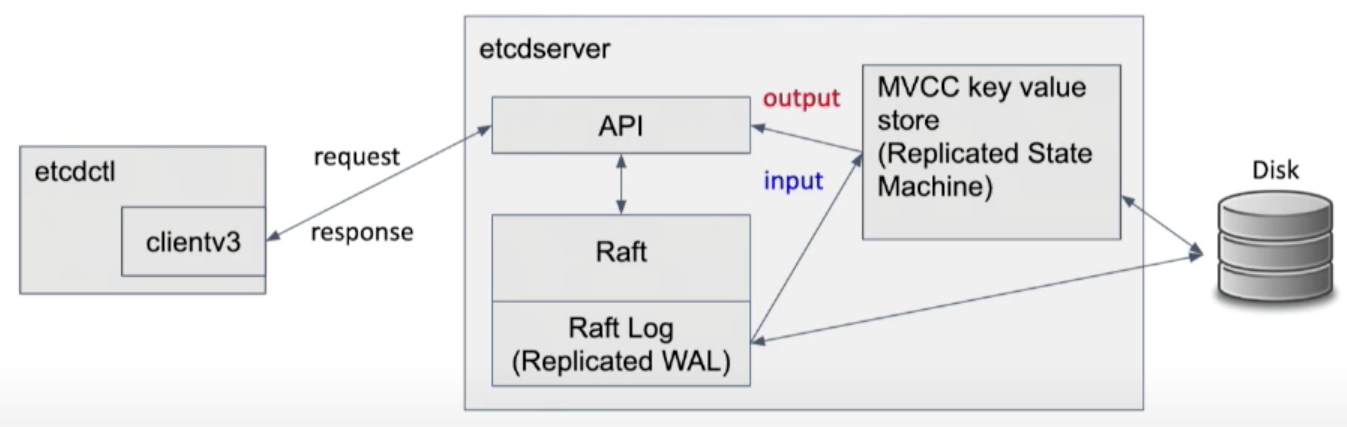
\includegraphics[width=0.8\textwidth]{figures/etcd.png}
    
    \framebreak
    
    \begin{block}{Installation}
        \begin{itemize}
            \item download release from \alert{\href{https://github.com/etcd-io/etcd/releases/}{github.com/etcd-io/etcd/releases}}
            %
            \item unpack the archive
            %
            \item add binaries to path
            %
            \item if you use Mac it is sufficient to run:\\
            %
            > \texttt{brew install etcd}
        \end{itemize}
    \end{block}
    
    \begin{block}{Docker images}
        There are public images on the Internet, for instance \alert{\href{https://hub.docker.com/r/bitnami/etcd/}{hub.docker.com/r/bitnami/etcd}}.
        \begin{itemize}
            \item \texttt{> docker pull bitnami/etcd}
            %
            \item \texttt{> docker run -d -it --rm --name etcd-server-1 ... bitnami/etcd}
        \end{itemize}
    \end{block}

    \framebreak
    
    \begin{block}{Hello world!}
        If you have installed etcd on your machine you can run \texttt{etcd} to start an etcd server.
        %
        Now you can use the command \texttt{etcdclt} to perform operation on the key-value store.
        %
        Run the following commands:
        \begin{itemize}
            %
            \item \texttt{> etcd}
            %
            \item \texttt{> etcdctl put greeting "Hello, etcd"}
            %
            \item \texttt{> etcdctl get greeting}
            %
            \item \texttt{> etcdctl del greeting}
        \end{itemize}
    %
    \end{block}
    
    \framebreak
    
    \begin{block}{etcd cluster}
        \begin{itemize}
            \item one etcd server on one container;
            %
            \item we must specify a configuration file to set up the cluster:\\
            %
            \texttt{-v etcd1.conf.yml:/opt/bitnami/etcd/conf/etcd.conf.yml}
        \end{itemize}
        %
        \lstinputlisting[morekeywords={var},basicstyle=\ttfamily\tiny]{./listings/conf.yml}
    \end{block}
    
    \framebreak
    
    \begin{block}{etcd cluster}
        Full command to run a docker etcd server container:\\
        %
        \lstinputlisting[language=bash,morekeywords={var},basicstyle=\ttfamily\tiny]{./listings/docker-run.txt}
    \end{block}
    
    \centering
    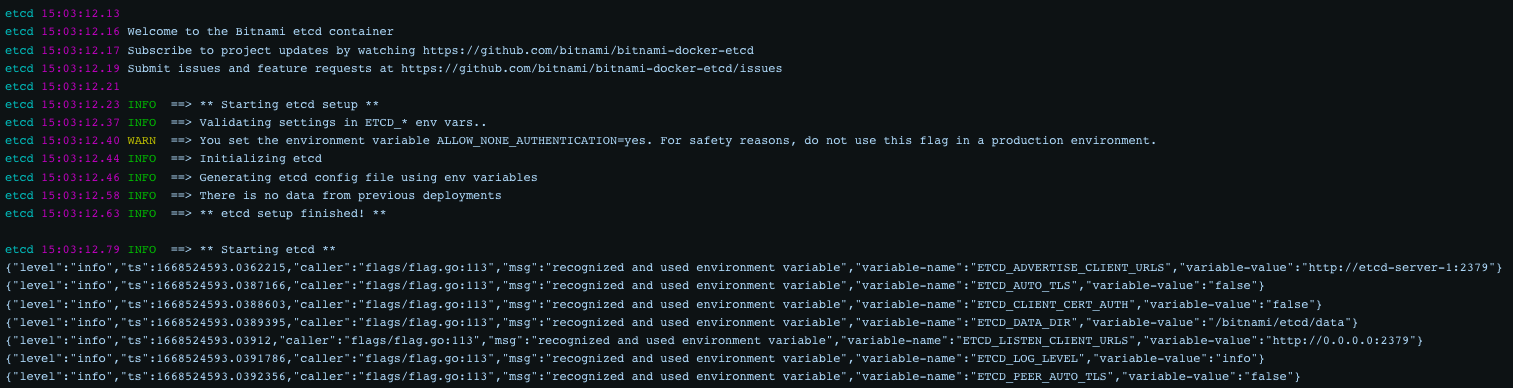
\includegraphics[width=\textwidth]{figures/docker-run-output.png}
    
\end{frame}

\begin{frame}[allowframebreaks]{jetcd}
    
    \begin{block}{About jetcd (\href{https://github.com/etcd-io/jetcd}{github.com/etcd-io/jetcd})}
        jetcd is a Java client for etcd (v3).
        %
        We will use it to build a quite simple multi-user chat client.
    \end{block}
    %
    \begin{block}{Gradle dependency}
        \lstinputlisting[language=kotlin,morekeywords={var},basicstyle=\ttfamily\tiny]{./listings/gradle-dep.txt}
    \end{block}

    \framebreak
    
    \begin{block}{jetcd main classes (\href{https://javadoc.io/doc/io.etcd/jetcd-core/latest/index.html}{documentation here})}
        \begin{itemize}
            \item \alert{\texttt{Client}}: an etcd client that can communicate to etcd servers.
            %
            When building a client it is necessary to specify the endpoints (etcd servers);
            %
            \item \alert{\texttt{KV}}: key-value client to perform actions on the KV store ( \texttt{put()},  \texttt{get()},  \texttt{delete()}).
            %
            You can get a \texttt{KV} client form an ectd  \texttt{Client} by calling the method \texttt{getKVClient()};
            %
            \item \alert{\texttt{Watch}}: a client for watching keys via method \texttt{watch()}.
            %
            You can get a \texttt{Watch} client form an ectd  \texttt{Client} by calling the method \texttt{getWatchClient()};
        \end{itemize}
    \end{block}
    
\end{frame}


\begin{frame}[allowframebreaks]{Exercise}
    
    \begin{block}{Breacking news}
        \begin{itemize}
            \item From this laboratory (included!) there won't be any mandatory activity.
        \end{itemize}
    \end{block}
    %
    \begin{block}{What we are going to do}
        We implement an etcd client for a group chat.
        %
        The client should be able to connect to etcd server(s) of the same cluster.
        %
        After the connection is established, clients can exchange messages with each-others.\\
        %
        Repository: \alert{\href{https://dvcs.apice.unibo.it/pika-lab/courses/ds/ay2223/lab-7}{dvcs.apice.unibo.it/pika-lab/courses/ds/ay2223/lab-7}}
    \end{block}

    \framebreak
    
    \begin{block}{Client behaviour}
        \begin{itemize}
            \item client should connect to etcd server(s);
            %
            \item client read from an input stream and \emph{put} a value (message) on the key-value store;
            %
            \item client \emph{watch} the key to handle events, the client should output the value of an event on an output stream.
            %
            So, the output should include client's messages and messages of other clients.
            %
            \item we don't care about old messages, if a client connects after some messages have already put to the key-value store we can ignore them.
        \end{itemize}
    \end{block}
\end{frame}


%===============================================================================
\section*{}
%===============================================================================

%/////////
\frame{\titlepage}
%/////////

%===============================================================================
\section*{\refname}
%===============================================================================

%%%%
\setbeamertemplate{page number in head/foot}{}
%/////////
%\begin{frame}[c,noframenumbering]{\refname}
\begin{frame}[t,allowframebreaks,noframenumbering]{\refname}
%	\tiny
	\scriptsize
%	\footnotesize
	\bibliographystyle{apalike-AMS}
	\bibliography{sd-lab-consensus}
\end{frame}
%/////////

%%%%%%%%%%%%%%%%%%%%%%%%%%%%%%%%%%%%%%%%%%%%%%%%%%%%%%%%%%%%%%%%%%%%%%%%%%%%%%%%
\end{document}
%%%%%%%%%%%%%%%%%%%%%%%%%%%%%%%%%%%%%%%%%%%%%%%%%%%%%%%%%%%%%%%%%%%%%%%%%%%%%%%%
